% Version 2020-12-15
% update – 161114 by Ken Arroyo Ohori: made spacing closer to Word template throughout, put proper quotes everywhere, removed spacing that could cause labels to be wrong, added non-breaking and inter-sentence spacing where applicable, removed explicit newlines
% update – 010819 by Dennis Wittich: made spacing and font size closer to Word template, updated references and refernces style
% update – 042319 by Dennis Wittich: font size of captions set to 'small', first author names are shortened, hyphenation fixed
% update – 010620 by Dennis Wittich: Footnotes alignment set to left
% update - 151220 by Clement Mallet: Template adapted for double blind full paper submissions
% update - 060321 by Christian Heipke: Template refined for double blind full paper submissions
% update - 090921 by Christian Heipke: Template refined for double blind full paper submissions

\documentclass{isprs} % isprs class modified 23-04-2019 (Dennis Wittich)
\usepackage{subfigure}
\usepackage{setspace}
\usepackage{geometry} % added 27-02-2014 Markus Englich
\usepackage{epstopdf}
\usepackage[labelsep=period]{caption}  % added 14-04-2016 Markus Englich - Recommendation by Sebastian Brocks
\usepackage[british]{babel} 
\usepackage[hang]{footmisc}
\usepackage[hidelinks]{hyperref}
\def\footnotemargin{1em} % added 08-01-2020 Dennis Wittich

%\usepackage[authoryear]{natbib}
%\def\bibhang{0pt}

\geometry{a4paper, top=25mm, left=20mm, right=20mm, bottom=25mm, headsep=10mm, footskip=12mm} % added 27-02-2014 Markus Englich
%\usepackage{enumitem}

%\usepackage{isprs}
%\usepackage[perpage,para,symbol*]{footmisc}

%\renewcommand*{\thefootnote}{\fnsymbol{footnote}}
\captionsetup{justification=centering,font=normal} % thanks to Niclas Borlin 05-05-2016
\captionsetup[figure]{font=small} % added 23-04-2019 Dennis Wittich
\captionsetup[table]{font=small} % added 23-04-2019 Dennis Wittich

% For RMD compat
\newlength{\cslhangindent}
\setlength{\cslhangindent}{1.5em}
\newlength{\csllabelwidth}
\setlength{\csllabelwidth}{3em}
\newlength{\cslentryspacingunit} % times entry-spacing
\setlength{\cslentryspacingunit}{\parskip}
\newenvironment{CSLReferences}[2] % #1 hanging-ident, #2 entry spacing
 {% don't indent paragraphs
  \setlength{\parindent}{0pt}
  % turn on hanging indent if param 1 is 1
  \ifodd #1
  \let\oldpar\par
  \def\par{\hangindent=\cslhangindent\oldpar}
  \fi
  % set entry spacing
  \setlength{\parskip}{#2\cslentryspacingunit}
 }%
 {}
\usepackage{calc}
\newcommand{\CSLBlock}[1]{#1\hfill\break}
\newcommand{\CSLLeftMargin}[1]{\parbox[t]{\csllabelwidth}{#1}}
\newcommand{\CSLRightInline}[1]{\parbox[t]{\linewidth - \csllabelwidth}{#1}\break}
\newcommand{\CSLIndent}[1]{\hspace{\cslhangindent}#1}
\setlength{\emergencystretch}{3em} % prevent overfull lines
\providecommand{\tightlist}{%
  \setlength{\itemsep}{0pt}\setlength{\parskip}{0pt}}

% https://stackoverflow.com/questions/41052687/rstudio-pdf-knit-fails-with-environment-shaded-undefined-error

\usepackage{booktabs} % To thicken table lines

\begin{document}

\title{Exploring jittering and routing options for converting OD data into route networks: towards accurate estimates of movement at the street level}
\date{}


% KAO: Remove extra spacing
% Anonymous submissions, authors' names should not be visible
\author{
R. Lovelace \textsuperscript{1}\thanks{Corresponding author}
, R. Félix \textsuperscript{2}, 
D. Carlino \textsuperscript{3}
}

% KAO: Remove extra newline
% Anonymous submissions, authors' affiliations should not be visible
\address{
\textsuperscript{1} Institute for Transport Studies, University of Leeds, UK - r.lovelace@leeds.ac.uk \\
\textsuperscript{2} CERIS, Instituto Superior Técnico, University of Lisbon, Portugal - rosamfelix@tecnico.ulisboa.pt \\
\textsuperscript{3} Alan Turing Institute, UK - dcarlino@turing.ac.uk
}

% If the corresponding author is NOT the final author, always add a % space before the subsequent comma, i.e.
% first author name\textsuperscript{a,}\thanks{Corresponding author} , % second author name \textsuperscript{b}, etc.
% thanks to Niclas Borlin 05-05-2016


\commission{IV, }{YY} %This field is optional. If filled, XX and YY should be replaced by adequate numbers. See https://www2.isprs.org/commissions/
\workinggroup{IV/4} %This field is optional.
\icwg{}   %This field is optional.

% KAO: Use times symbol
\abstract{

% These guidelines are provided for preparation of \textbf{full papers} submitted to ISPRS events (Congress, Geospatial Week, Symposia, smaller events). If the double-blind review process leads to acceptance, they will be either published in the series of Volumes of The International Archives of the Photogrammetry, Remote Sensing and Spatial Information Sciences or of The ISPRS Annals of the Photogrammetry, Remote Sensing and Spatial Information Sciences.  
Origin-Destination (OD) datasets provide vital information on how people travel betewen areas in many cities, regions and countries worldwide. OD datasets are usually represented geographically with straight lines or routes between zone centroids. For active travel, this geographic representation has substantial limitations, especially when zone origins and centroids are large: only using a single centroid origin/destination for each large zone results in sparse route networks covering only a small fraction of likely walking and cycling routes. This paper implements and explores the use of jittering and different routing options to overcome this limitation, thereby adding value to aggregate OD data to support investment in sustainable transport infrastructure. The route network results --- generated from on an open dataset representing cycling trips in Lisbon, Portugal --- were compared with a ground-truth dataset from 67 count locations distributed throughout the city. This approach enabled exploration of which jittering parameters and routing options lead to the most accurate route network results approximating the real geographic distribution of cycling trips in the study area. We found that jittering and disaggregating OD data, combined with routing using low level of taffic stress (quieter) preferences resulted in the most accurate route networks. We conclude that a combined approach involing 1) jittering with intermediate levels of disaggregation and 2) careful selection of routing options can lead to much more realistic route networks than using established OD processing techniques. The methods can be deployed to support evidence-based investment in strategic cycling and other sustainable transport networks in cities worldwide.
}

\keywords{Origin-Destination data, Methods, Jittering, Active transport, Road network, Validation.}

\maketitle

%\saythanks % added 28-02-2014 Markus Englich

% \section{MANUSCRIPT}\label{MANUSCRIPT}
 
% KAO: Sloppy spacing ensures non-overfull lines. Can be removed if this is not an issue.
\sloppy

% \subsection{General Instructions}\label{sec:General Instructions}
% 
% The paper should have the following structure: 
% 
% %\itemize
% \begin{enumerate}
% \setlength\itemsep{0em}\setlength\parskip{0em}\setlength\topsep{0em}\setlength\partopsep{0em}\setlength\parsep{0em} 
% \item{Title of the paper} 
% \item{Authors and affiliation, rendered \textbf{anonymous} }
% \item{Keywords (6--8 words)}
% \item{Abstract (100--250 words)}
% \item{Introduction}
% \item{Main body}
% \item{Conclusions}
% \item{Acknowledgements, rendered \textbf{anonymous}}
% \item{References}
% \item{Appendix (if applicable)}
% \end{enumerate}
% 
% % KAO: Use proper quotes
% Full papers \textbf{submitted for double-blind review} must not contain any information which makes it possible to identify the authors. In particular, names and affiliations must be removed from the manuscript submitted for review. Also sentences such as ''As we have shown in previous work (Author\_x, 20xx)'' are to be avoided. Instead use a formulation such as ''Author\_x (20xx) has shown ...''. Note that submissions which have not been appropriately anonymised may be subject to immediate rejection.\\
% In case, the contribution has been accepted for publication, a camera-ready manuscript must be submitted at the due date. In this camera-ready manuscript the name(s) and affiliation(s) of the authors(s) must be identified, and acknowledgements can be personalized.
% % In Section~\ref{MANUSCRIPT} we present related work
% %\newpage            
% \subsection{Page Layout, Spacing and Margins}\label{sec:Page Layout, Spacing and Margins}
% 
% The paper must be compiled in one column for the Title and Abstract and in two columns for all subsequent text. All text should be single-spaced, unless otherwise stated. Left and right justified typing is preferred.
% 
% 
% \subsection{Preparation in electronic form}\label{sec:Preparation in electronic form}
% 
% % KAO: Remove newline
% To assist authors in preparing their contributions, styleguides are 
% provided in Word and/or LaTeX on the ISPRS web Page, see: http://www.isprs.org/documents/orangebook/app5.aspx.
% 
% 
% 
% \subsection{Length and Font}\label{sec:Length and Font}
% 
% All manuscripts, except Invited Papers are limited to a length of approximately eight (8) single-spaced pages (A4 size), including abstracts, figures, tables and references. ISPRS Invited Papers are limited to approximately twelve (12) pages. In any case, the minimum length is six (6) pages. The font type Times New Roman with a size of nine (9) points is to be used.
% 
% % KAO: Removed spacing before label: can cause references to be wrong
% \begin{table}[h]
% 	\centering
% 		\begin{tabular}{|l|c|c|}\hline
% 			Setting&\multicolumn{2}{c|}{A4 size page}\\\hline
% 			  &mm&inches\\
% 			 Top&25&1.0\\
% 			 Bottom&25&1.0\\
% 			 Left&20&0.8\\
% 			 Right&20&0.8\\
% 			 Column Width&82&3.2\\
% 			 Column Spacing&6&0.25\\\hline
% 		\end{tabular}
% 	\caption{Margin settings for A4 size page.}
% \label{tab:Margin_settings}
% \end{table}
% 
% \section{TITLE AND ABSTRACT BLOCK}\label{sec:TITLE AND ABSTRACT BLOCK}
% 
% \subsection{Title}\label{sec:Title}
% 
% The title should appear centred in bold capital letters, at the top of the first page of the paper with a size of twelve (12) points and single-spacing. Author(s) name(s), affiliation and mailing address should be masked. They will only appear in the final version if the paper is accepted either in the ISPRS Annals or Archives.
% 
% \subsection{ISPRS Affiliation (optional)}\label{sec:ISPRS Affiliation (optional)}
% 
% % KAO: Use proper quotes
% For those authors affiliated with a specific Commission and/or Working Group of ISPRS, a separate title may be entered. The title should be centred in bold type after one blank line below the author’s affiliation, i.e. Commission~\#, Working Group~\#. The Commission number shall be Roman and the Working Group number should be the Commission Roman number, slash, WG Arabic number (see example above).
% 
% 
% \subsection{Key Words}\label{sec:Key Words}
% 
% % KAO: Use proper quotes and dash
% Leave two lines blank, then type \textbf{``KEY WORDS:''}
% in bold capital letters, followed by 5--8 key words. Note that ISPRS does not provide a set 
% list of key words any longer. Therefore, include those key words which you would 
% use to find a paper with content you are preparing.
% 
% 
% \subsection{Abstract}\label{sec:Abstract}
% 
% % KAO: Use proper quotes and dash
% Leave two blank lines under the key words. Type \textbf{``ABSTRACT:''}
% flush left in bold Capitals followed by one blank line. Start now
% with a concise Abstract (100--250 words) which presents briefly the
% content and very importantly, the news and results of the paper in
% words understandable also to non-specialists. 
% 
% 
% \section{MAIN BODY OF TEXT}\label{sec:MAIN BODY OF TEXT}
% 
% Type text single-spaced, \textbf{with} one blank line between paragraphs and 
% following headings. Start paragraphs flush with left margin.

\hypertarget{introduction}{%
\section{Introduction}\label{introduction}}

Origin-destination (OD) datasets provide information on aggregate travel patterns between zones and geographic entities, and can be obtained from a wide range of sources making them one of the most commonly used geographic inputs in applied transport planning (Alexander et al. 2015).
OD datasets are often `implicitly geographic', containing identification codes of the geographic objects from which trips start and end.
Exact coordinates of origins and destinations are provided in this way for good reasons: historically computational resources constrained analysis options, meaning that data reduction (by converting thousands of travel survey responses into a more compact aggregate OD dataset) was important; and privacy considerations prevent the disclosure of exact trip start and end points (Boyce and Williams 2015).

A common approach to converting OD datasets to geographic entities, for example represented using the simple features standard (Open Geospatial Consortium Inc 2011) and saved in file formats such as GeoPackage and GeoJSON, is to represent each OD record as a straight line between zone centroids.
This approach to representing OD datasets on the map has been since at least the 1950s (Boyce and Williams 2015) and --- despite the development of various methods to add value to OD datasets by sampling start and end points and `connectors' withing each zone (Lovelace, Félix, and Carlino 2022), discussed below --- centroid-based geographic representations of OD data are still dominant (Rae 2009; Tennekes and Chen 2021).
Before explaining the methods, it is worth defining terms:

\begin{itemize}
\item
  \textbf{Origins}: locations of trip departure, typically stored as ID codes linking to zones
\item
  \textbf{Destinations}: trip destinations, also stored as ID codes linking to zones
\item
  \textbf{Attributes}: the number of trips made between each `OD pair' and additional attributes such as route distance between each OD pair
\item
  \textbf{Jittering}: The combined process of `splitting' OD pairs representing many trips into multiple `sub OD' pairs (disaggregation) and assigning origins and destinations to multiple unique points within each zone
\end{itemize}

Beyond simply visualising aggregate travel patterns, centroid-based geographic desire lines are also used as the basis of many transport modelling processes.
The following steps can be used to convert OD datasets into route networks, in a process that can generate nationally scalable results (Morgan and Lovelace 2020):

\begin{itemize}
\item
  OD data converted into centroid-based geographic desire lines
\item
  Calculation of routes for each desire line, with start and end points at zone centroids
\item
  Aggregation of routes into route networks, with values on each segment representing the total amount of travel (`flow') on that part of the network, using functions such as \texttt{overline()} in the open source R package \texttt{stplanr} (Lovelace and Ellison 2018)
\end{itemize}

This approach is tried and tested:
the OD \(\rightarrow\) desire line \(\rightarrow\) route \(\rightarrow\) route network processing pipeline forms the basis of the route network results in the Propensity to Cycle Tool, an open source and publicly available map-based web application for informing strategic cycle network investment, `visioning' and prioritisation (Lovelace et al. 2017; Goodman et al. 2019).
However, the approach has some key limitations:

\begin{itemize}
\item
  Flows are concentrated on transport network segments leading to zone centroids, creating distortions in the results and preventing the simulation of the diffuse networks that are particularly important for walking and cycling
\item
  The results are highly dependent on the size and shape of geographic zones used to define OD data
\item
  The approach is inflexible, providing few options to people who want to use valuable OD datasets in different ways
\end{itemize}

To overcome these limitations, methods of `jittering' OD data have been developed (Lovelace, Félix, and Carlino 2022).
While the results from analysis of route networks generated from jittered OD data in that paper were promising, the input datasets were small and technique was not evaluated with reference to ground truth data.
This raised the question ``Are the jittered results measurably better when compared with counter datasets on the network?'' (Lovelace, Félix, and Carlino 2022).

This question was partially addressed during a presentation and subsequent proceedings published as part of the GISRUK conference (Lovelace et al. 2022).
However, the input dataset used for that conference paper was small and overly focussed on Edinburgh.
Furthermore, only a single routing option was used, raising the question:
what is the relative importance of geographic OD data pre-processing (jittering) and routing options when preparing route networks to support strategic sustainable transport plans?
We set out to address this question in this paper.

\hypertarget{software-and-reproducibility}{%
\subsection{Software and reproducibility}\label{software-and-reproducibility}}

In this paper present results generated using the \texttt{odjitter} Rust crate.
We developed an interface to R in the \texttt{odjitter} R package (not on CRAN at the time of writing) that can form the basis of a implementations in other languages that interface with the highly efficient Rust implementation.
The results presented in this paper are fully reproducible.
See the paper's GitHub repository at \url{https://github.com/Robinlovelace/foss4g22/} for implementation details and to reproduce the results.

\hypertarget{approach}{%
\section{Approach}\label{approach}}

\hypertarget{jittering}{%
\subsection{Jittering}\label{jittering}}

Jittering represents a comparatively simple --- compared with `connector' based methods (Jafari et al. 2015) --- approach is to OD data preprocessing.
For each OD pair, the jittering approach consists of the following steps for each OD pair (provided it has required inputs of a disaggregation threshold, a single number greater than one, and sub-points from which origin and destination points are located):

\begin{enumerate}
\def\labelenumi{\arabic{enumi}.}
\tightlist
\item
  Checks if the number of trips (for a given `disaggregation key', e.g.~`walking') is greater than the disaggregation threshold.
\item
  If so, the OD pair is disaggregated. This means being divided into as many pieces (`sub-OD pairs') as is needed, with trip counts divided by the number of sub-OD pairs, for the total to be below the disaggregation threshold.
\item
  For each sub-OD pair (or each original OD pair if no disaggregation took place) origin and destination locations are randomly sampled from sub-points which optionally have weights representing relative probability of trips starting and ending there.
\end{enumerate}

This approach has been implemented efficiently in the Rust crate \texttt{odjitter}, the source code of which can be found at \url{https://github.com/dabreegster/odjitter}.

\hypertarget{case-study}{%
\subsection{Case study}\label{case-study}}

Lisbon, Portugal, is a city with about half million residents. By 2018, when a mobility survey was carried on, and only about 0.5\% of trips were made by bicycle. However, the investments in cycling infrastructure, reaching 150 km of cycling network in 2021, and the implementation of a dock-based bike-sharing system had a major impact on cycling levels (Félix, Cambra, and Moura 2020).

Cyclists' counts are performed yearly from 2017 to 2021 at more than 65 locations in Lisbon during morning and afternoon peak hours (8-10 am and 5-7 pm). In 2021, these were carried out in October.
The 67 locations, shown in Figure \ref{lisbonmap}, were chosen considering to the existent and planned
cycling infrastructure, and places where there was no cycling infrastructure, but had already some presence
of cyclists.

\begin{figure}

{\centering 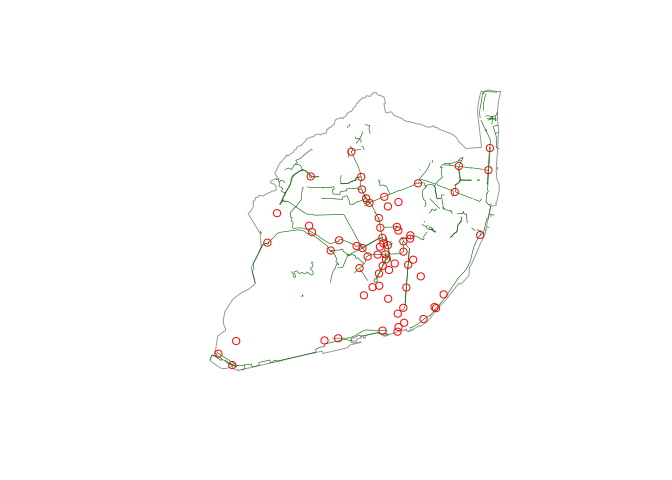
\includegraphics[width=1\linewidth]{README_files/figure-latex/lisbonmap-1} 

}

\caption{\label{lisbonmap}Cycling infrastructure in Lisbon as October 2021 and location of cyclists' counters.}\label{fig:lisbonmap}
\end{figure}

\hypertarget{methods}{%
\subsection{Methods}\label{methods}}

We use data from a mobility survey (Instituto National de Estatística 2018) at district level (Lisbon has 24 districts), including 4955 daily bicycle trips, represented by 122 desire lines.
Cycling count data includes 26464 passings in the total of the 67 locations (one trip may pass at more than one location).

Routes were computed using \href{https://cyclestreets.net}{\emph{CycleStreets}}, which relies on 2022 road network from OpenStreetMap, using \href{https://ipeagit.github.io/r5r/}{\texttt{r5r} engine} (Pereira et al. 2021), and using \emph{Google Maps} service, for routing comparison.

Regarding the routing options, CycleStreets provides 3 options of cycling routes: ``fastest'', ``balanced'' and ``quietest'', while r5r uses the Level of Traffic Stress (LTS), ranging from 1 - less bicycle friendly, to 4 - more bicycle friendly (Mekuria, Furth, and Nixon 2012). Google Maps does not provide such profile options for bicycle routing.
In this research we compared CycleStreets' ``quietest'' and ``fastest'' modes, and LTS 2 and 4.

This was an iterative process, an not all options were tested due to the computational requirements. We started by generating routes with CycleStreets for the 3 routing profiles and for unjittered, jittered with no disagregation, and jittered with disagregation level of 500 trips. Then we compared the results with routes generated by r5r, for 2 levels of traffic stress (2 and 4), and with routes generated by Google. Other jittering disagregation level of 200 trips was also compared with the previous results, for routes generated with CycleStreets (``quietest'' profile) and for routes generated with r5r (LTS 2).

Results were then assessed. Count data was compared with the resulting route networks (with information on bike trips at each segment level, from the mobility survey data) by taking the value of the nearest segment, and using a R\textsuperscript{2} correlation fit.

\hypertarget{results}{%
\section{Results}\label{results}}

We generated route networks based on a range of different jittering parameters and routing options.
The results presented in this section not only report estimates of model-counter fit but also provide indication of the type of networks generated, though route network maps.
Figures \ref{poltlisbon1}, \ref{poltlisbon2} and \ref{poltlisbon3} show the difference between desire lines with centroids approach and the jittering approach, for bike trips in Lisbon.

\begin{figure}

{\centering 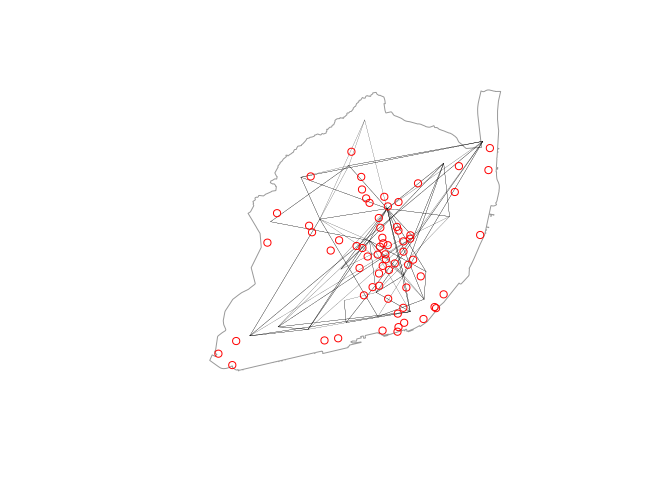
\includegraphics[width=1\linewidth]{README_files/figure-latex/jitteredoverview1-1} 

}

\caption{\label{poltlisbon1}Trips represented with desire lines from centroids of 24 areas. The red circles represent the counters locations.}\label{fig:jitteredoverview1}
\end{figure}

\begin{figure}

{\centering 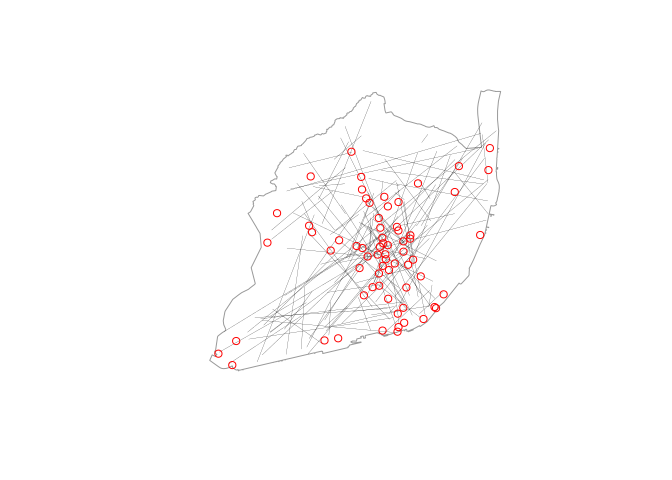
\includegraphics[width=1\linewidth]{README_files/figure-latex/jitteredoverview2-1} 

}

\caption{\label{poltlisbon2}Trips represented with jittered desire lines, with no disagregation.}\label{fig:jitteredoverview2}
\end{figure}

\begin{figure}

{\centering 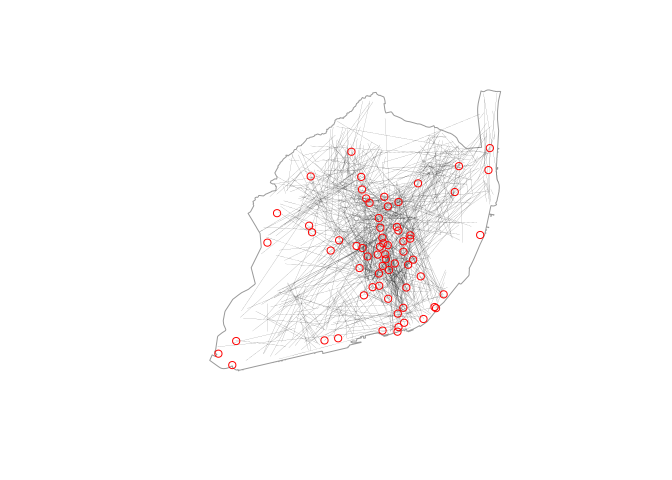
\includegraphics[width=1\linewidth]{README_files/figure-latex/jitteredoverview3-1} 

}

\caption{\label{poltlisbon3}Trips represented with jittered desire lines, with disagregation of 500 trips.}\label{fig:jitteredoverview3}
\end{figure}

Figures \ref{map1}, \ref{map2}, \ref{map3} and \ref{map4} show examples of route networks from unjittered OD pairs, and jittered OD pairs with disagregation level of 500 trips, for differen routing providers, and the counters location.

\begin{figure}

{\centering 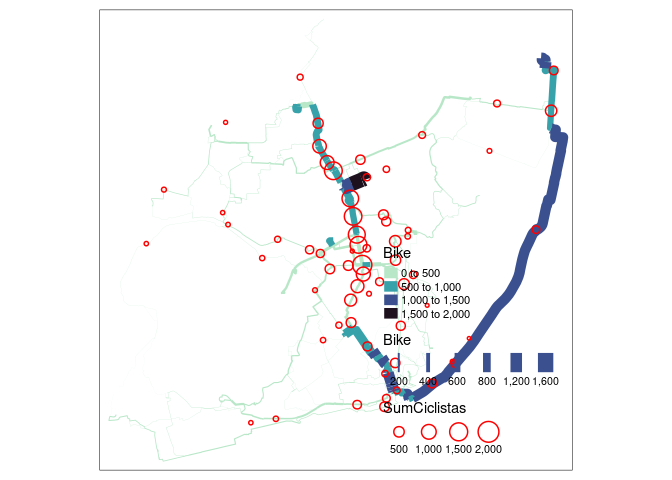
\includegraphics[width=1\linewidth]{README_files/figure-latex/map1-1} 

}

\caption{\label{map1}Route network from unjittered desire lines, with routes from CycleStreets, in quietest routing option.}\label{fig:map1}
\end{figure}

\begin{figure}

{\centering 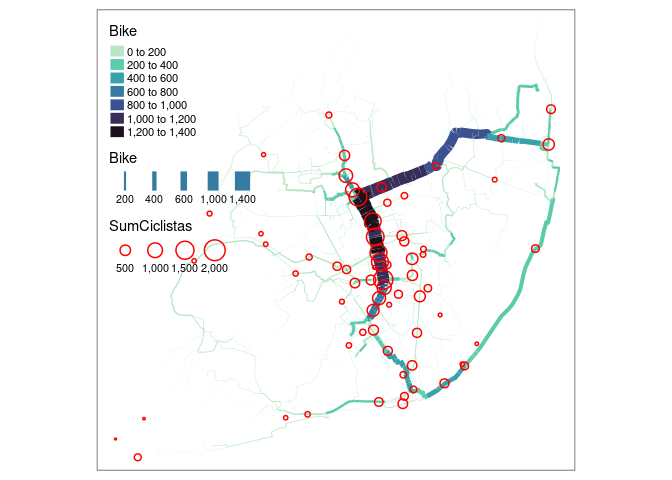
\includegraphics[width=1\linewidth]{README_files/figure-latex/map2-1} 

}

\caption{\label{map2}Route network from jittered desire lines with disagregation of 500 trips, with routes from CycleStreets, in quietest routing option.}\label{fig:map2}
\end{figure}

\begin{figure}

{\centering 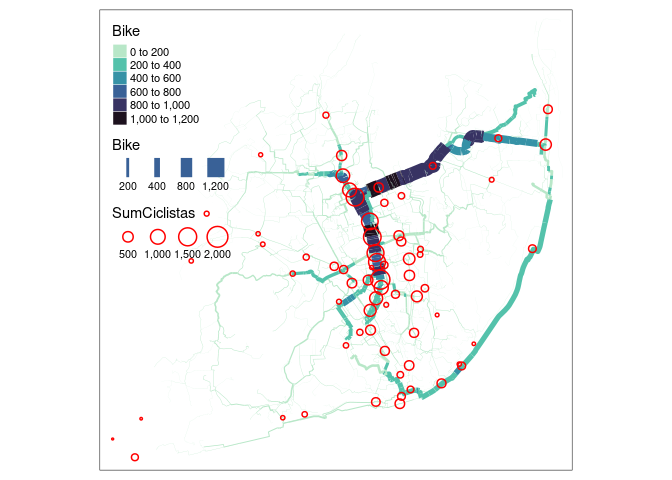
\includegraphics[width=1\linewidth]{README_files/figure-latex/map3-1} 

}

\caption{\label{map3}Route network from jittered desire lines with disagregation of 500 trips, with routes from r5r, level of traffic stress 2 (quiet) routing option.}\label{fig:map3}
\end{figure}

\begin{figure}

{\centering 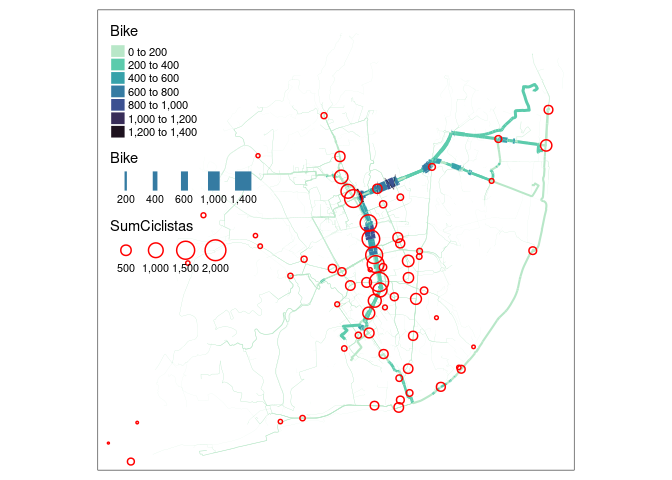
\includegraphics[width=1\linewidth]{README_files/figure-latex/map4-1} 

}

\caption{\label{map4}Route network from jittered desire lines with disagregation of 500 trips, with routes from Google.}\label{fig:map4}
\end{figure}

\begin{figure}

{\centering 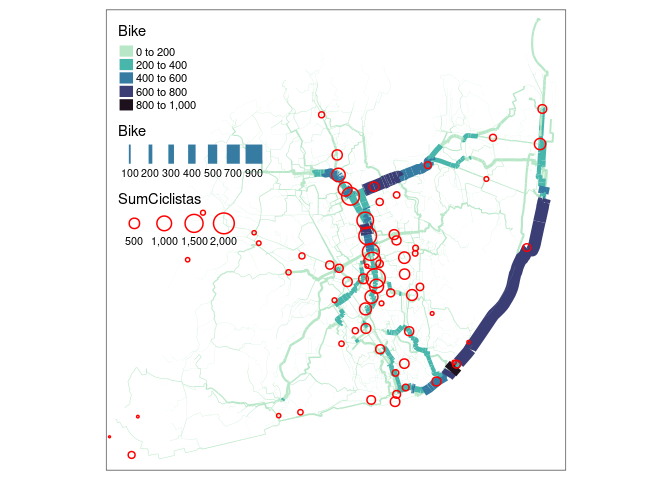
\includegraphics[width=1\linewidth]{README_files/figure-latex/map5-1} 

}

\caption{\label{map5}Route network from jittered desire lines with disagregation of 200 trips, with routes from r5r, level of traffic stress 2 (quiet) routing option.}\label{fig:map5}
\end{figure}

When comparing the route network with unjittered desire lines (Figure \ref{map1}) with the jittered ones (Figures \ref{map2}, \ref{map3} and \ref{map4}), we may find that the route networks from jittered desire lines are more diffuse, and not concentrated in a few routes. For cycling and walking, this bring more realistic routes for this transport modes. Nevertheless, we are aware that routing options ``quiet'', and LTS 2 (quieter than LTS4), have a higher weight in using the existing cycling network infrastructure, and then the resulting route network can be similar to the cycling network silhouette (see Figure \ref{lisbonmap}). In fact, cyclists tend to opt for a cycling infrastructure when it is available, even if it compromises the directness of their trips (Broach, Dill, and Gliebe 2012).
It is also noticed that ``Fastest'' and LTS4 routing option does not have a good fit with the counting data, when compared with the ``Quietest'' and LTS2.

Regarding the different disagregation levels, a route network build from a jittering disagregation of 200 trips is shown in Figure \ref{map5}, with a more diffuse network.

Although useful for visualizing the complex and spatially diffuse reality of travel patterns, we found that the most valuable use of jittering is as a pre-processing stage before routing and route network generation.
Route networks generated from jittered desire lines are more diffuse, and potentially more realistic, than centroid-based desire lines.

We also found that the approach, implemented in Rust and with bindings to R and Python (in progress), is fast.
Benchmarks show that the approach can `jitter' desire lines representing millions of trips in a major city in less than a minute on consumer hardware.

We also found that the results of jittering depend on the geographic input datasets representing start points and trip attractors, and the use of weights.

Table \ref{tableresults} shows the counter data vs modeled route network fit, with different routing and jittering parameters. We can observe that jittered OD pairs provide a better fit result, with disagregation.

\begin{table}

\caption{\label{tab:unnamed-chunk-10}\label{tableresults}Results showing counter/model fit for route networks generated from different routing and jittering parameters}
\centering
\begin{tabular}[t]{llrr}
\toprule
Jittering & Routing & Nrow & R-Squared\\
\midrule
Unjittered & quietest & 122 & 0.23\\
Unjittered & balanced & 122 & 0.22\\
Unjittered & fastest & 122 & 0.10\\
Unjittered & LTS2 & 122 & 0.35\\
Unjittered & LTS4 & 122 & 0.04\\
\addlinespace
Jittered, no disaggregation & quietest & 122 & 0.26\\
Jittered, no disaggregation & balanced & 122 & 0.11\\
Jittered, no disaggregation & fastest & 122 & 0.00\\
\addlinespace
Jittered, 500 disaggregation & quietest & 799 & 0.50\\
Jittered, 500 disaggregation & balanced & 799 & 0.42\\
Jittered, 500 disaggregation & fastest & 799 & 0.08\\
Jittered, 500 disaggregation & LTS2 & 799 & 0.54\\
Jittered, 500 disaggregation & LTS4 & 799 & 0.14\\
Jittered, 500 disaggregation & Google & 799 & 0.25\\
\addlinespace
Jittered, 200 disaggregation & quietest & 1895 & 0.54\\
Jittered, 200 disaggregation & LTS2 & 1895 & 0.54\\
\bottomrule
\end{tabular}
\end{table}

A higher jittered disagregation level (200 trips) does not bring a better fit against a lower disagregation level of 500 trips. This might be explained but the routing profile used in the routing engines, and the location of the cycling counters - most of them at the existing cycling infrastructure.
Although a more diffuse route network is expected in active transportation modes, the available data and computed routes are usually closer to where cycling infrastructure exists. Other data should be used to validate this hypothesis, such as a more diffuse cyclists' counters location, or/and the actual cyclist's routes --- for example, bike sharing trips routes, despite their access is not usually guaranteed for research purposed.

The results from our analysis suggest that investment in cycle infrastructure is particularly important in a few key locations where cycling potential is high yet provision is poor.
These locations are highlighted in Figure \ref{fig:segments}, which was generated using information from three key sources:

\begin{itemize}
\tightlist
\item
  Estimates of cycling potential, generated using the jittering \(\rightarrow\) routing \(\rightarrow\) route network methods presented in this paper.
\item
  Estimates of quietness of links on the network, computed with the open source cyclestreets R package (Desjardins et al. 2022).
\item
  Local knowledge, which was used to visually inspect the resulting networks and identify key `severance' points in the network (Mindell and Anciaes 2020).
\end{itemize}

\begin{figure}

{\centering 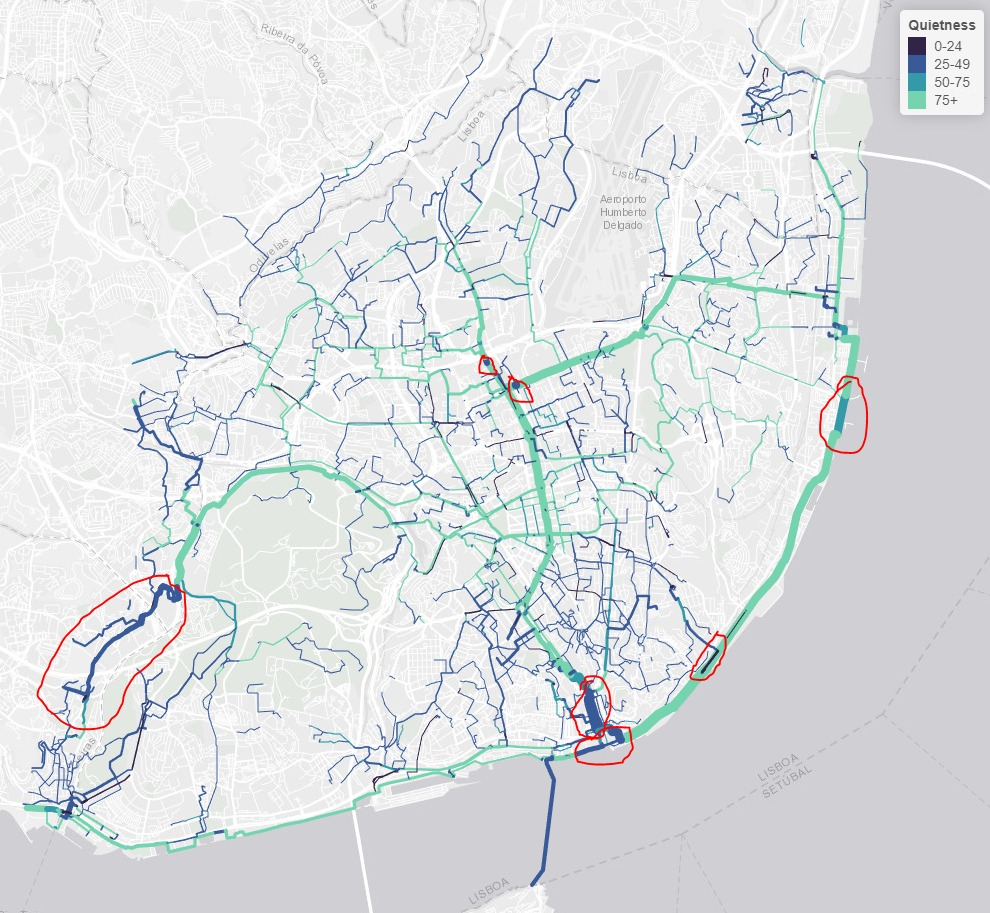
\includegraphics[width=1\linewidth]{figures/priority-segments} 

}

\caption{Segments on the transport network of Lisbon where investment in new cycling infrastructure should be prioritised according to the route networks generated using methods presented in this paper, alongside local knowledge.}\label{fig:segments}
\end{figure}

Figure \ref{fig:segments} highlights the policy relevant nature of this research.
A key finding is that, combined with local knowledge and detailed data on existing transport infrastructure, which can be used to generate metrics such as Level of Traffic Stress (LTS) (Wang et al. 2016) and Cycling Level of Service (CLoS) (Deegan 2015), route networks generated from jittered, disaggregated, and appropriated routed OD data can help prioritise investment where it is most needed.
Results were presented to stakeholders working in the local area who said that these new results would support their investment plans.

The overall result was the finding that OD jittering methods first developed by Lovelace, Félix, and Carlino (2022) are not enough on their own to generate accurate route networks.
Jittering leads to more spatially diffuse route networks than networks generated from the common approach of routing from and to zone centroids.
However, the results presented in this section show that careful consideration of routing options is needed in addition to evidence-based selection of jittering parameters.

\hypertarget{conclusion}{%
\section{Conclusion}\label{conclusion}}

Building on previous work (Lovelace, Félix, and Carlino 2022), we have explored the relative importance of jittering and routing options.
As with previous work, we found that jittering leads to more spatially diverse geographic representations of travel between zones.
Because the results were generated only for a single city, and because we did not explore the full parameter space (alternative subpoint weighting parameters in the jittering process are discussed below), we cannot draw specific and universally applicable conclusions about the optimal settings for accurate route network generation in other cities.
It should be remembered that route networks and cycling preferences vary from city to city (Buehler and Dill 2016).
However, although our findings were based on a single case study, Lisbon, Portugal, the findings have implications for future work using OD data to support evidence-based investment in sustainable transport infrastructure (e.g. Vybornova et al. 2022).
The overall finding is that both 1) careful translation of OD data to geographic start and end locations and disaggregation and 2) careful selection of routing options are needed \emph{in combination} to ensure that route networks derived from OD data are diffuse and accurate.

Accurate route network representations of transport systems are needed to support investment in a variety of transport interventions (Morgan and Lovelace 2020).
We have focused in this study on cycleway network because a complete cycle network represents one of the most cost-effective ways to reduce car dependence and associated environmental, economic, social and health costs (Wałdykowski, Adamczyk, and Dorotkiewicz 2022).
Cycleway \emph{networks}, rather than simply isolated routes or other geographically sparse interventions, are vital for successful active travel investment (Buehler and Dill 2016).
Our results are therefore highly policy relevant, adding value to established methods of adding value to OD data to support sustainable transport planning (Lovelace et al. 2017; Larsen, Patterson, and El-Geneidy 2013; Mohammed and Oke 2022).

The research presented in this paper is not without limitations.
We did not explore the full range of jittering and routing options available due to time and computational resource constraints.
Specifically, varying the type and weights of origin and destination subpoints, as advocated in Lovelace, Félix, and Carlino (2022), could lead to improved fit.
This would require filtering the subpoints used to include only certain types of nodes on the road network (all vertices on the road network were used as the basis for both origin subpoints and destination subpoints in this study, see \href{https://github.com/dabreegster/odjitter}{documentation} in the \texttt{odjitter} Rust crate for details).
Future work could explore the use of including only residential roads, or increasing the weight associated with residential roads, in the origin subpoints, for example.
Likewise, destination subpoints and associated weights could be altered to prioritise key trip attractors such as schools and commercial centres.
Another limitation is the simplistic measure of accuracy used in this study.
Accuracy was inferred from goodness-of-fit between aggregated flow values at 67 counter locations and modeled flow on nearest segment on the network.
Future work could use alternative measures of fit such as root-mean-square error (RMSE) and more sophisticated ways of comparing observed counter values to modeled networked values, e.g.~using inverse distance weighted measures associated with links in close proximity to each counter, with empirically derived bandwidths.

More broadly, the quality of the underlying route network data is imperfect.
Efforts to improve the underlying OpenStreetMap data will continue to overcome this limitation, not just in Lisbon but worldwide (Barrington-Leigh and Millard-Ball 2017).
This will improve the results over time because all routing engines used in this study, except for Google's routing service, use OSM data.
Furthermore, alternative data sources and methods could be used to generate more accurate road networks (e.g. Leninisha and Vani 2015).
Future work should seek to test a wider range of jittering parameters in multiple case study areas with larger ground truth datasets.
Other fit measures, such as GEH or SQV statistics, may also be used to compare count data with simulated traffic volumes.

Despite these limitations, and the need for future academic work, the results are already useful.
Imperfect data-driven evidence is better than no data-driven data, especially when practitioners are aware of the mechanisms underlying route network level estimates of travel behavior such as those presented in this paper.
A benefit of the approach is that it based on open source software and reproducible code, allowing others to build on the methods (Lovelace, Parkin, and Cohen 2020).
Indeed, a next step building on directly on the research presented in this paper is to use the results to support strategic cycle network planning in Lisbon and the wider area.
In parallel to efforts to improve route network representations of transport systems we therefore advocate for the use of the approach presented in this paper, and related methods (e.g. Cooper 2018; Vybornova et al. 2022), to be implemented in support of more evidence-based investment in sustainable transport infrastructure at city, regional and national scales worldwide.

\hypertarget{references}{%
\section*{References}\label{references}}
\addcontentsline{toc}{section}{References}

\hypertarget{refs}{}
\begin{CSLReferences}{1}{0}
\leavevmode\vadjust pre{\hypertarget{ref-alexander_validation_2015}{}}%
Alexander, Lauren, Shan Jiang, Mikel Murga, and Marta C Gonz. 2015. {``Validation of Origin-Destination Trips by Purpose and Time of Day Inferred from Mobile Phone Data.''} \emph{Transportation Research Part B: Methodological}, 1--20. \url{https://doi.org/10.1016/j.trc.2015.02.018}.

\leavevmode\vadjust pre{\hypertarget{ref-barrington-leigh_world_2017}{}}%
Barrington-Leigh, Christopher, and Adam Millard-Ball. 2017. {``The World's User-Generated Road Map Is More Than 80\% Complete.''} \emph{PLOS ONE} 12 (8): e0180698. \url{https://doi.org/10.1371/journal.pone.0180698}.

\leavevmode\vadjust pre{\hypertarget{ref-boyce_forecasting_2015}{}}%
Boyce, David E., and Huw C. W. L. Williams. 2015. \emph{Forecasting {Urban Travel}: {Past}, {Present} and {Future}}. {Edward Elgar Publishing}.

\leavevmode\vadjust pre{\hypertarget{ref-Broach2012}{}}%
Broach, Joseph, Jennifer Dill, and John Gliebe. 2012. {``Where Do Cyclists Ride? {A} Route Choice Model Developed with Revealed Preference {GPS} Data.''} \emph{Transportation Research Part A: Policy and Practice} 46 (10): 1730--40. \url{https://doi.org/10.1016/j.tra.2012.07.005}.

\leavevmode\vadjust pre{\hypertarget{ref-buehler_bikeway_2016}{}}%
Buehler, Ralph, and Jennifer Dill. 2016. {``Bikeway {Networks}: {A Review} of {Effects} on {Cycling}.''} \emph{Transport Reviews} 36 (1): 9--27. \url{https://doi.org/10.1080/01441647.2015.1069908}.

\leavevmode\vadjust pre{\hypertarget{ref-cooper_predictive_2018}{}}%
Cooper, Crispin H. V. 2018. {``Predictive Spatial Network Analysis for High-Resolution Transport Modeling, Applied to Cyclist Flows, Mode Choice, and Targeting Investment.''} \emph{International Journal of Sustainable Transportation} 0 (0): 1--11. \url{https://doi.org/10.1080/15568318.2018.1432730}.

\leavevmode\vadjust pre{\hypertarget{ref-deegan_cycling_2015}{}}%
Deegan, Brian. 2015. {``Cycling Infrastructure in {London}.''} \emph{Proceedings of the Institution of Civil Engineers - Engineering Sustainability} 169 (3): 92--100. \url{https://doi.org/10.1680/jensu.15.00001}.

\leavevmode\vadjust pre{\hypertarget{ref-desjardins_correlates_2022}{}}%
Desjardins, Elise, Christopher D. Higgins, Darren M. Scott, Emma Apatu, and Antonio Páez. 2022. {``Correlates of Bicycling Trip~Flows in {Hamilton}, {Ontario}: Fastest, Quietest, or Balanced Routes?''} \emph{Transportation} 49 (3): 867--95. \url{https://doi.org/10.1007/s11116-021-10197-1}.

\leavevmode\vadjust pre{\hypertarget{ref-felix_build_2020a}{}}%
Félix, Rosa, Paulo Cambra, and Filipe Moura. 2020. {``Build It and Give `Em Bikes, and They Will Come: {The} Effects of Cycling Infrastructure and Bike-Sharing System in {Lisbon}.''} \emph{Case Studies on Transport Policy} 8 (June): 672--82. \url{https://doi.org/10.1016/j.cstp.2020.03.002}.

\leavevmode\vadjust pre{\hypertarget{ref-goodman_scenarios_2019}{}}%
Goodman, Anna, Ilan Fridman Rojas, James Woodcock, Rachel Aldred, Nikolai Berkoff, Malcolm Morgan, Ali Abbas, and Robin Lovelace. 2019. {``Scenarios of Cycling to School in {England}, and Associated Health and Carbon Impacts: {Application} of the {`{Propensity} to {Cycle Tool}'}.''} \emph{Journal of Transport \& Health} 12 (March): 263--78. \url{https://doi.org/10.1016/j.jth.2019.01.008}.

\leavevmode\vadjust pre{\hypertarget{ref-IMOB}{}}%
Instituto National de Estatística. 2018. {``Mobilidade e Funcionalidade Do Território Nas {Áreas Metropolitanas} Do {Porto} e de {Lisboa}: 2017.''} {Lisboa}. \url{https://www.ine.pt/xportal/xmain?xpid=INE\&xpgid=ine_publicacoes\&PUBLICACOESpub_boui=349495406\&PUBLICACOESmodo=2\&xlang=pt}.

\leavevmode\vadjust pre{\hypertarget{ref-jafari_investigation_2015}{}}%
Jafari, Ehsan, Mason D. Gemar, Natalia Ruiz Juri, and Jennifer Duthie. 2015. {``Investigation of {Centroid Connector Placement} for {Advanced Traffic Assignment Models} with {Added Network Detail}.''} \emph{Transportation Research Record: Journal of the Transportation Research Board} 2498 (June): 19--26. \url{https://doi.org/10.3141/2498-03}.

\leavevmode\vadjust pre{\hypertarget{ref-larsen_build_2013}{}}%
Larsen, Jacob, Zachary Patterson, and Ahmed El-Geneidy. 2013. {``Build It. {But} Where? {The} Use of Geographic Information Systems in Identifying Locations for New Cycling Infrastructure.''} \emph{International Journal of Sustainable Transportation} 7 (4): 299--317. \url{http://www.tandfonline.com/doi/abs/10.1080/15568318.2011.631098}.

\leavevmode\vadjust pre{\hypertarget{ref-leninisha_water_2015}{}}%
Leninisha, Shanmugam, and Kaliaperumal Vani. 2015. {``Water Flow Based Geometric Active Deformable Model for Road Network.''} \emph{ISPRS Journal of Photogrammetry and Remote Sensing} 102 (April): 140--47. \url{https://doi.org/10.1016/j.isprsjprs.2015.01.013}.

\leavevmode\vadjust pre{\hypertarget{ref-lovelace_stplanr_2018}{}}%
Lovelace, Robin, and Richard Ellison. 2018. {``Stplanr: {A Package} for {Transport Planning}.''} \emph{The R Journal} 10 (2): 7--23. \url{https://doi.org/10.32614/RJ-2018-053}.

\leavevmode\vadjust pre{\hypertarget{ref-lovelace_assessing_2022}{}}%
Lovelace, Robin, Rosa Félix, Dustin Carlin, and Roger Beecham. 2022. {``Assessing Methods for Generating Route Networks from Origin-Destionation Data: Jittering, Routing, and Visualisation.''} Presented at the 30th {Annual Geographical Information Science Research UK} ({GISRUK}), {Liverpool, United Kingdom}, March 29. \url{https://doi.org/10.5281/zenodo.6410196}.

\leavevmode\vadjust pre{\hypertarget{ref-lovelace_jittering_2022b}{}}%
Lovelace, Robin, Rosa Félix, and Dustin Carlino. 2022. {``Jittering: {A Computationally Efficient Method} for {Generating Realistic Route Networks} from {Origin-Destination Data}.''} \emph{Findings}, April, 33873. \url{https://doi.org/10.32866/001c.33873}.

\leavevmode\vadjust pre{\hypertarget{ref-lovelace_propensity_2017}{}}%
Lovelace, Robin, Anna Goodman, Rachel Aldred, Nikolai Berkoff, Ali Abbas, and James Woodcock. 2017. {``The {Propensity} to {Cycle Tool}: {An} Open Source Online System for Sustainable Transport Planning.''} \emph{Journal of Transport and Land Use} 10 (1). \url{https://doi.org/10.5198/jtlu.2016.862}.

\leavevmode\vadjust pre{\hypertarget{ref-lovelace_open_2020}{}}%
Lovelace, Robin, John Parkin, and Tom Cohen. 2020. {``Open Access Transport Models: {A} Leverage Point in Sustainable Transport Planning.''} \emph{Transport Policy} 97 (October): 47--54. \url{https://doi.org/10.1016/j.tranpol.2020.06.015}.

\leavevmode\vadjust pre{\hypertarget{ref-mekuria2012low}{}}%
Mekuria, Maaza C, Peter G Furth, and Hilary Nixon. 2012. {``Low-Stress Bicycling and Network Connectivity.''} \url{https://scholarworks.sjsu.edu/cgi/viewcontent.cgi?article=1073\&context=mti_publications}.

\leavevmode\vadjust pre{\hypertarget{ref-mindell_chapter_2020}{}}%
Mindell, Jennifer S., and Paulo R. Anciaes. 2020. {``Chapter Seven - {Transport} and Community Severance.''} In \emph{Advances in {Transportation} and {Health}}, edited by Mark J. Nieuwenhuijsen and Haneen Khreis, 175--96. {Elsevier}. \url{https://doi.org/10.1016/B978-0-12-819136-1.00007-3}.

\leavevmode\vadjust pre{\hypertarget{ref-mohammed_origindestination_2022}{}}%
Mohammed, Mohammed, and Jimi Oke. 2022. {``Origin-Destination Inference in Public Transportation Systems: {A} Comprehensive Review.''} \emph{International Journal of Transportation Science and Technology}, March. \url{https://doi.org/10.1016/j.ijtst.2022.03.002}.

\leavevmode\vadjust pre{\hypertarget{ref-morgan_travel_2020}{}}%
Morgan, Malcolm, and Robin Lovelace. 2020. {``Travel Flow Aggregation: Nationally Scalable Methods for Interactive and Online Visualisation of Transport Behaviour at the Road Network Level.''} \emph{Environment \& Planning B: Planning \& Design}, July. \url{https://doi.org/10.1177/2399808320942779}.

\leavevmode\vadjust pre{\hypertarget{ref-ogcopengeospatialconsortiuminc_opengis_2011}{}}%
Open Geospatial Consortium Inc, (OGC). 2011. {``{OpenGIS Implementation Specification} for {Geographic} Information - {Simple} Feature Access - {Part} 1: {Common} Architecture.''} OGC 06-103r4. {(OGC) Open Geospatial Consortium Inc.} \url{https://www.ogc.org/standards/sfa}.

\leavevmode\vadjust pre{\hypertarget{ref-pereira_r5r_2021}{}}%
Pereira, Rafael H. M., Marcus Saraiva, Daniel Herszenhut, Carlos Kaue Vieira Braga, and Matthew Wigginton Conway. 2021. {``R5r: {Rapid Realistic Routing} on {Multimodal Transport Networks} with {R}{\textsuperscript{5}} in {R}.''} \emph{Findings}, March, 21262. \url{https://doi.org/10.32866/001c.21262}.

\leavevmode\vadjust pre{\hypertarget{ref-rae_spatial_2009}{}}%
Rae, Alasdair. 2009. {``From Spatial Interaction Data to Spatial Interaction Information? {Geovisualisation} and Spatial Structures of Migration from the 2001 {UK} Census.''} \emph{Computers, Environment and Urban Systems} 33 (3): 161--78. \url{https://doi.org/10.1016/j.compenvurbsys.2009.01.007}.

\leavevmode\vadjust pre{\hypertarget{ref-tennekes_design_2021}{}}%
Tennekes, Martijn, and Min Chen. 2021. {``Design {Space} of {Origin-Destination Data Visualization}.''} \emph{Computer Graphics Forum} 40 (3): 323--34. \url{https://doi.org/10.1111/cgf.14310}.

\leavevmode\vadjust pre{\hypertarget{ref-vybornova_automated_2022a}{}}%
Vybornova, Anastassia, Tiago Cunha, Astrid Gühnemann, and Michael Szell. 2022. {``Automated {Detection} of {Missing Links} in {Bicycle Networks}.''} \emph{Geographical Analysis} n/a (n/a). \url{https://doi.org/10.1111/gean.12324}.

\leavevmode\vadjust pre{\hypertarget{ref-waldykowski_sustainable_2022}{}}%
Wałdykowski, Piotr, Joanna Adamczyk, and Maciej Dorotkiewicz. 2022. {``Sustainable {Urban Transport}---{Why} a {Fast Investment} in a {Complete Cycling Network Is Most Profitable} for a {City}.''} \emph{Sustainability} 14 (1, 1): 119. \url{https://doi.org/10.3390/su14010119}.

\leavevmode\vadjust pre{\hypertarget{ref-wang_does_2016}{}}%
Wang, Haizhong, Matthew Palm, Chen Chen, Rachel Vogt, and Yiyi Wang. 2016. {``Does Bicycle Network Level of Traffic Stress ({LTS}) Explain Bicycle Travel Behavior? {Mixed} Results from an {Oregon} Case Study.''} \emph{Journal of Transport Geography} 57: 8--18.

\end{CSLReferences}

% \subsection{Headings}\label{sec:Headings}
% 
% % KAO: Remove explicit newlines in this section
% Major headings are to be centred, in bold capitals without 
% underlining, after two blank lines and followed by a one blank line.
% 
% Type subheadings flush with the left margin in bold upper case and lower 
% case letters. Subheadings are on a separate line between two single blank lines.
% 
% Subsubheadings are to be typed in bold upper case and lower case letters 
% after one blank line flush with the left margin of the page, with text 
% following on the same line. Subsubheadings may be followed by a period 
% or colon, they may also be the first word of the paragraph's sentence.
% 
% Use decimal numbering for headings and subheadings.
% 
% 
% \subsection{Footnotes}\label{sec:Footnotes}
% 
% Mark footnotes in the text with a number (1); use consecutive numbers for following footnotes. Place footnotes at the bottom of the page, separated from the text above it by a horizontal line.
% 
% 
% \subsection{Illustrations and Tables}\label{sec:Illustrations and Tables}
% 
% \subsubsection{Placement:}\label{sec:Placement}
% 
% Figures must be placed in the appropriate location in the document, 
% as close as practicable to the reference of the figure in the text. 
% While figures and tables are usually aligned horizontally on the page, 
% large figures and tables sometimes need to be turned on their sides. 
% If you must turn a figure or table sideways, please be sure that the 
% top is always on the left-hand side of the page.
% 
% 
% \subsubsection{Captions:}\label{sec:Captions}
% 
% All captions should be typed in upper and lower case letters, 
% centred directly beneath the illustration. Use single spacing if they 
% use more than one line. All captions are to be numbered consecutively, 
% e.g. Figure~1, Figure~2, Figure~3, ..  and Table~1, Table~2, Table~3, ...
% 
% % KAO: Remove spacing before label: can cause reference to be wrong
% \begin{figure}[ht!]
% \begin{center}
% 		\includegraphics[width=1.0\columnwidth]{figures/test_sites/fig1.eps}
% 	\caption{Figure placement and numbering.}
% \label{fig:figure_placement}
% \end{center}
% \end{figure}
% 
% 
% \subsubsection{Copyright:}\label{sec:Copyright}
% 
% % KAO: Inter-sentence spacing
% If your article contains any copyrighted illustrations or imagery, 
% please include a statement of copyright such as: \copyright~SPOT Image Copyright 20xx 
% (fill in year), CNES\@. It is the author's responsibility to obtain any necessary 
% copyright permission. After publication, your article is distributed under \underline{the Creative 
% Commons Unported License} and you retain the copyright.
% 
% 
% \subsection{Equations, Symbols and Units}\label{sec:Equations, Symbols and Units}
% 
% \subsubsection{Equations:}\label{sec:Equations}
% 
% Equations should be numbered consecutively throughout the contribution. The equation 
% number is enclosed in parentheses and placed flush right. Leave one blank lines 
% before and after equations: 
% 
% 
% \begin{equation}\label{equ:1}
% 	x = x_0 -c \frac{X - X_0}{Z - Z_0}; y = y_0 -c \frac{Y - Y_0}{Z - Z_0},
% \end{equation}
% 
% 
% \subsubsection{Symbols and Units:}\label{sec:Symbols and Units}
% Use the SI (Syst\`{e}me International) Units and Symbols. Unusual characters 
% or symbols should be explained in a list of nomenclature.
% 
% % KAO: Non-breaking space
% \subsection{References}\label{sec:References}
% References should be cited in the text, thus~\cite{smith1987rep}, and listed in alphabetical order in the reference section. The following arrangements should be used:
% 
% % KAO: Use proper quotes and non-breaking space
% \subsubsection{References from Journals:} 
% Journals should be cited like~\cite{smith1987} or~\cite{michalis2008}. Names of journals can be abbreviated according to the ``International List of Periodical Title Word Abbreviations''. In case of doubt, write names in full.
% 
% \subsubsection{References from Books:} 
% Books should be cited like~\cite{foerstner2016}.
% 
% \subsubsection{References from other Literature:}
% Other literature should be cited like~\cite{smith1987rep} and~\cite{smith2000}.
% 
% \subsubsection{References from Websites:}
% References from the internet should be cited like~\cite{chan2017} and~\cite{maas2017}. Use ofpersistent identifiers such as the Digital Object Identifier (DOI) rather than URLs is strongly advised. In this case last date of visiting the website can be omitted, as the identifier will not change.
% 
% \subsubsection{References from Research Data:}
% References from research data should be cited like~\cite{dubayah2013}.
% 
% \subsubsection{References from Software Projects:}
% References to a software project as a high level container including multiple versions of the software should be cited like~\cite{grass2017}.
% 
% \subsubsection{References from Software Versions:}
% References to a specific software version should be cited like~\cite{grass2015}.
% 
% \subsubsection{References from Software Project Add-ons:}
% References to a specific software add-on to a software project should be cited like~\cite{lennert2017}.
% 
% \subsubsection{References from Software Repository:}
% References from software repositories should be cited like~\cite{gago2016}.

\section*{ACKNOWLEDGEMENTS}\label{ACKNOWLEDGEMENTS}
We thank Lisbon Municipal Government and Transport Infrastructure Ireland for funding this research.

% {
% 	\begin{spacing}{1.17}
% 		\normalsize
% 		\bibliography{ISPRSguidelines_authors} % Include your own bibliography (*.bib), style is given in isprs.cls
% 	\end{spacing}
% }
% 
% 
% \section*{APPENDIX (Optional)}\label{APPENDIX}
% 
% Any additional supporting data may be appended, provided the paper does not exceed the limits given above. 


\end{document}
